This chapter reports results under the within-subject protocol: every model is trained and tested on the same participant. Per-modality and naive late-fusion figures involve no model selection; every learned-fusion figure is leak-free (Section~\ref{sec:learned_fusion_results}).

\section{Single-Modality Performance}

\subsection{Pilot}
The encoders were first run on participants 1--3. With a deliberately short budget (AST 2 + 2 epochs, ViT 1 + 1, EEGNet 50), audio and vision were already well above chance, but EEG averaged 24.4\%, essentially chance (Table~\ref{tab:day1_smoke_test}). That result led to the two EEGNet defects described in Chapter~\ref{chap:engineering_challenges}. After fixing them and moving to the full budget, the same three participants reached the accuracies in Table~\ref{tab:day2_full_budget}, with EEG at 50.6\%.

\begin{table}[htbp]
\centering
\small
\caption{Pilot, short training budget (AST 2 + 2, ViT 1 + 1, EEGNet 50 epochs). Chance is 20\%.}
\label{tab:day1_smoke_test}
\begin{tabular}{c c c c}
\hline
\textbf{Participant} & \textbf{Audio} & \textbf{Vision} & \textbf{EEG} \\
\hline
01 & 49.2\% & 62.5\% & 30.8\% \\
02 & 69.2\% & 69.2\% & 20.8\% \\
03 & 50.8\% & 80.0\% & 21.7\% \\
\hline
Mean & 56.4\% & 70.6\% & 24.4\% \\
\hline
\end{tabular}
\end{table}

\begin{table}[htbp]
\centering
\small
\caption{Pilot, full budget after the EEGNet fixes. Change from Table~\ref{tab:day1_smoke_test}: audio $+4.7$, vision $+5.0$, EEG $+26.2$ points.}
\label{tab:day2_full_budget}
\begin{tabular}{c c c c}
\hline
\textbf{Participant} & \textbf{Audio} & \textbf{Vision} & \textbf{EEG} \\
\hline
01 & 55.8\% & 62.5\% & 44.2\% \\
02 & 71.7\% & 80.8\% & 54.2\% \\
03 & 55.8\% & 83.3\% & 53.3\% \\
\hline
Mean & 61.1\% & 75.6\% & 50.6\% \\
\hline
\end{tabular}
\end{table}

The 26.2-point EEG gain mixes two changes---the fixes and the longer schedule---that these runs cannot separate; a 50-epoch rerun of participant~1 after the softmax fix alone moved it by only about one point. Either way, EEG needed to be clearly above chance before it could contribute anything to fusion.

\subsection{All 42 Participants}
Table~\ref{tab:full_rollout_accuracy} gives the 42-participant means. Each encoder beats the corresponding EAV baseline: audio by 20.4 points, vision by 21.8 and EEG by 7.2. Vision is the strongest modality (74.6\%), audio intermediate (57.1\%) and EEG weakest (43.9\%), which is consistent with a facial-emotion model pre-trained on large image collections, a general audio model adapting to emotional speech, and an EEG model trained from scratch on 280 trials. Chapter~\ref{chap:crosssubject} shows that much of vision's lead is participant-specific.

\begin{table}[htbp]
\centering
\small
\caption{Within-subject means over 42 participants. Fusion heads are leak-free (final epoch of a fixed 80-epoch schedule; Section~\ref{sec:learned_fusion_results}).}
\label{tab:full_rollout_accuracy}
\begin{tabular}{p{5.0cm} p{3.6cm} p{5.1cm}}
\hline
\textbf{Method} & \textbf{Mean accuracy} & \textbf{Comparison} \\
\hline
Audio (AST) & 57.1\% & $+20.4$ over SCNN (36.7\%) \\
Vision (ViT) & 74.6\% & $+21.8$ over DeepFace (52.8\%) \\
EEG (EEGNet) & 43.9\% & $+7.2$ over EEGNet (36.7\%) \\
Naive late fusion & 77.5\% & $+2.9$ over vision ($p = 0.020$) \\
Concat-MLP & 79.96\% & $+2.48$ over naive ($p_{\mathrm{Holm}} = 0.031$) \\
Attention & 76.75\% & $-0.73$ vs naive (n.s.) \\
Attention + modality dropout & 79.80\% & $+3.06$ over attention ($p_{\mathrm{Holm}} < 10^{-3}$) \\
\hline
\end{tabular}
\end{table}

\textbf{RQ1 answer:} Yes. Every modality is classified well above the published EAV baselines within-subject.

\section{Naive Late Fusion}
\label{sec:naive_late_fusion_results}

Averaging the three encoders' class probabilities (Section~\ref{sec:naive_method}) gives 77.5\% over 42 participants, 2.9 points above vision alone. The paired Wilcoxon test over participants is significant ($W = 251.5$, $p = 0.020$, rank-biserial $r = +0.42$), with 29 of the 41 untied participants favouring fusion. On the three pilot participants the gain looked larger (81.9\% against 75.6\%, $+6.3$ points), but those three happened to be comparatively easy; the 42-participant figure is the estimate to use.

\textbf{RQ2 answer:} Yes. Fusing the three modalities improves on the best single one, by 2.9 points for plain averaging. The leak-free learned heads reach 76.8--80.0\% (Section~\ref{sec:learned_fusion_results}), 2.2 to 5.4 points above the vision mean, though those differences were not tested against vision directly.

\section{Learned Fusion: Attention and Concatenation}
\label{sec:learned_fusion_results}
\label{sec:cross_attention_results}
\label{sec:concat_mlp_results}

\textbf{Terminology.} Following common usage, ``cross-attention fusion'' in this report refers to the \texttt{TrimodalAttentionFusion} module, which implements attention-based fusion as self-attention over three modality tokens (Section~\ref{sec:fusion_design_rationale}); ``attention'' is used as shorthand.

\textbf{Leak-free figures.} The Pre-Thesis~II report chose each fusion head's epoch by its test accuracy, which inflated the learned-fusion figures by 5.3 to 7.5 points (Section~\ref{sec:audit_selection}). Every learned-fusion figure here is instead taken at the final epoch of a fixed schedule trained on all 280 training trials, with no selection of any kind.

The attention module is compared with the concatenation MLP of Section~\ref{sec:concat_baseline} (1.35 million parameters against 2.29 million), which separates the value of attention from the value of learning a fusion at all. Both use the settings of Table~\ref{tab:fusion_hyperparameters}.

\begin{table}[htbp]
\centering
\small
\caption{Leak-free within-subject fusion accuracy, 42 participants. CI: 10{,}000-sample bootstrap over participants. SD: across participants.}
\label{tab:within_means}
\begin{tabular}{lcccc}
\hline
\textbf{Method} & \textbf{Mean} & \textbf{95\% CI} & \textbf{SD} & \textbf{Range} \\
\hline
Concat-MLP              & 79.96\% & [77.5, 82.3] & 0.078 & 60.8--95.8 \\
Modality dropout (full) & 79.80\% & [77.2, 82.3] & 0.083 & 60.8--95.8 \\
Modality dropout (AV)   & 79.17\% & [76.7, 81.6] & 0.083 & 56.7--95.0 \\
Naive late fusion       & 77.48\% & [74.7, 80.2] & 0.091 & 59.2--94.2 \\
Cross-attention         & 76.75\% & [74.1, 79.4] & 0.086 & 58.3--91.7 \\
\hline
\end{tabular}
\end{table}

\begin{table}[htbp]
\centering
\small
\caption{Leak-free within-subject comparisons, paired Wilcoxon signed-rank over 42 participants. $p_{\mathrm{Holm}}$ is corrected within the 7-test family shown.}
\label{tab:within_tests}
\begin{tabular}{llcccc}
\hline
\textbf{A} & \textbf{B} & \textbf{$\Delta$} & \textbf{A better} & \textbf{$p$} & \textbf{$p_{\mathrm{Holm}}$} \\
\hline
Concat-MLP              & Naive late fusion & $+2.48$ pp & 29/42 & 0.0063 & 0.031 \\
Modality dropout (full) & Naive late fusion & $+2.32$ pp & 31/42 & 0.0085 & 0.034 \\
Modality dropout (AV)   & Naive late fusion & $+1.69$ pp & 27/42 & 0.098  & 0.29 \\
Cross-attention         & Naive late fusion & $-0.73$ pp & 20/42 & 0.41   & 0.83 \\
\hline
Concat-MLP              & Cross-attention   & $+3.21$ pp & 32/42 & 0.0017 & 0.010 \\
Modality dropout (full) & Cross-attention   & $+3.06$ pp & 32/42 & $4.4\times10^{-5}$ & $3.1\times10^{-4}$ \\
Concat-MLP              & Modality dropout (full) & $+0.16$ pp & 19/42 & 0.72 & 0.83 \\
\hline
\end{tabular}
\end{table}

Tables~\ref{tab:within_means} and~\ref{tab:within_tests} give the results. Three findings follow.

First, \textbf{plain cross-attention fusion does not beat naive late fusion} within-subject: 76.75\% against 77.48\%, a difference of $-0.73$ points that is not significant. The advantage reported in Pre-Thesis~II ($+2.7$ points) was an artefact of test-set epoch selection.

Second, \textbf{concat-MLP and modality-dropout fusion exceed naive late fusion by about 2.4 points}, but the margin is marginal: it is significant after Holm correction within the family of Table~\ref{tab:within_tests} ($p_{\mathrm{Holm}} = 0.031$ and 0.034) and within the four head-versus-naive tests alone (0.025 for both), but not within a larger family that also includes the validation-selected readouts (0.050 and 0.059; Section~\ref{sec:audit_selection}). It is reported as such and no conclusion rests on it.

Third, \textbf{concat-MLP beats cross-attention} by 3.21 points ($p_{\mathrm{Holm}} = 0.010$, 32 of 42 participants). With single pooled vectors per modality, the attention module's relational inductive bias has only three tokens to relate, and a direct non-linear map over the joint 2{,}496-dimensional feature space extracts more of the available cross-modal information. The same ordering reappears on unseen participants once their features are calibrated (Section~\ref{sec:cal_ranking}), so it is a property of this representation rather than of one protocol.

The attention architecture is nonetheless retained as the thesis's fusion design, for two reasons that do not depend on raw accuracy. It exposes named per-modality post-attention embeddings as outputs of \texttt{forward()}, the contract required by the Phase~2 temporal head (Section~\ref{sec:fusion_design_rationale}); and, as the next section shows, modality-dropout training closes its gap to concat-MLP entirely.

\section{Modality Dropout and Robustness}
\label{sec:modality_dropout_results}

Softhard modality dropout (Section~\ref{sec:modality_dropout}) trains the attention module on inputs in which, for each sample with probability 0.5, one randomly chosen modality is replaced by zeros and the remaining ones are rescaled. The trained model is then evaluated with all modalities present and with EEG zeroed---the audio-visual (AV) configuration of any user without an EEG headset.

\begin{table}[htbp]
\centering
\small
\caption{Modality-dropout model under different inference configurations. Leak-free figures are final-full. The Pre-Thesis~II figures were measured at the epoch that maximised full-modality \emph{test} accuracy and are shown only for the relative cost of removing each modality; their absolute values are inflated.}
\label{tab:robustness}
\begin{tabular}{lcc}
\hline
\textbf{Inference configuration} & \textbf{Leak-free} & \textbf{Pre-Thesis~II (test-selected epoch)} \\
\hline
Full (audio + vision + EEG) & 79.80\% & 84.7\% \\
AV only (EEG zeroed) & 79.17\% & 81.5\% \\
VE only (audio zeroed) & not measured & 79.7\% \\
AE only (vision zeroed) & not measured & 54.0\% \\
\hline
\end{tabular}
\end{table}

\textbf{Dropout makes attention competitive.} Modality-dropout training lifts the same attention architecture from 76.75\% to 79.80\%, a gain of 3.06 points ($p_{\mathrm{Holm}} = 3.1\times10^{-4}$, 32 of 42 participants), and leaves it tied with concat-MLP ($-0.16$ points, not significant). This is the largest reproducible architectural effect in the within-subject results. Randomly removing a modality during training forces each modality token to carry self-sufficient evidence, which acts as a regulariser on a module that otherwise over-fits 280 training trials.

\textbf{The zero-EEG path survives.} With EEG zeroed at inference, the dropout model reaches 79.17\%. Removing EEG costs it 0.63 points, which is not significant ($p_{\mathrm{Holm}} = 0.16$ in a separate two-test family), and the AV configuration still beats full-modality cross-attention trained without dropout by 2.42 points ($p_{\mathrm{Holm}} = 0.0043$, 26 of 42 participants).

\textbf{Vision dominates within-subject.} The Pre-Thesis~II configuration results, although inflated in absolute terms, measure all four configurations at the same epoch and so remain informative about relative importance: removing vision cost 30.7 points, against 5.0 for audio and 3.2 for EEG. Chapter~\ref{chap:crosssubject} shows that this dominance is largely participant identity, which does not transfer.

\textbf{RQ5 answer:} Yes. The modality-dropout model produces useful predictions with EEG zeroed at inference: 79.17\% within-subject, not significantly below its full-modality accuracy, and significantly above cross-attention trained without dropout even when that model has EEG. The cross-subject counterpart is reported in Sections~\ref{sec:cs_discussion} and~\ref{sec:cal_ranking}.

\section{Per-Class Performance}
\label{sec:per_class_results}

Figure~\ref{fig:per_class_metrics} reports per-class performance of the modality-dropout model over all 5{,}040 test trials. It was produced in Pre-Thesis~II from the test-selected epoch, so its absolute values are inflated (by 7.5 points on average for this model; Table~\ref{tab:audit_leakfree}); leak-free per-trial predictions were not saved by the re-evaluation, so it cannot be regenerated. It is retained for the relative difficulty of the classes only.

\begin{figure}[htbp]
\centering
\IfFileExists{images/fig_6_4_per_class.png}{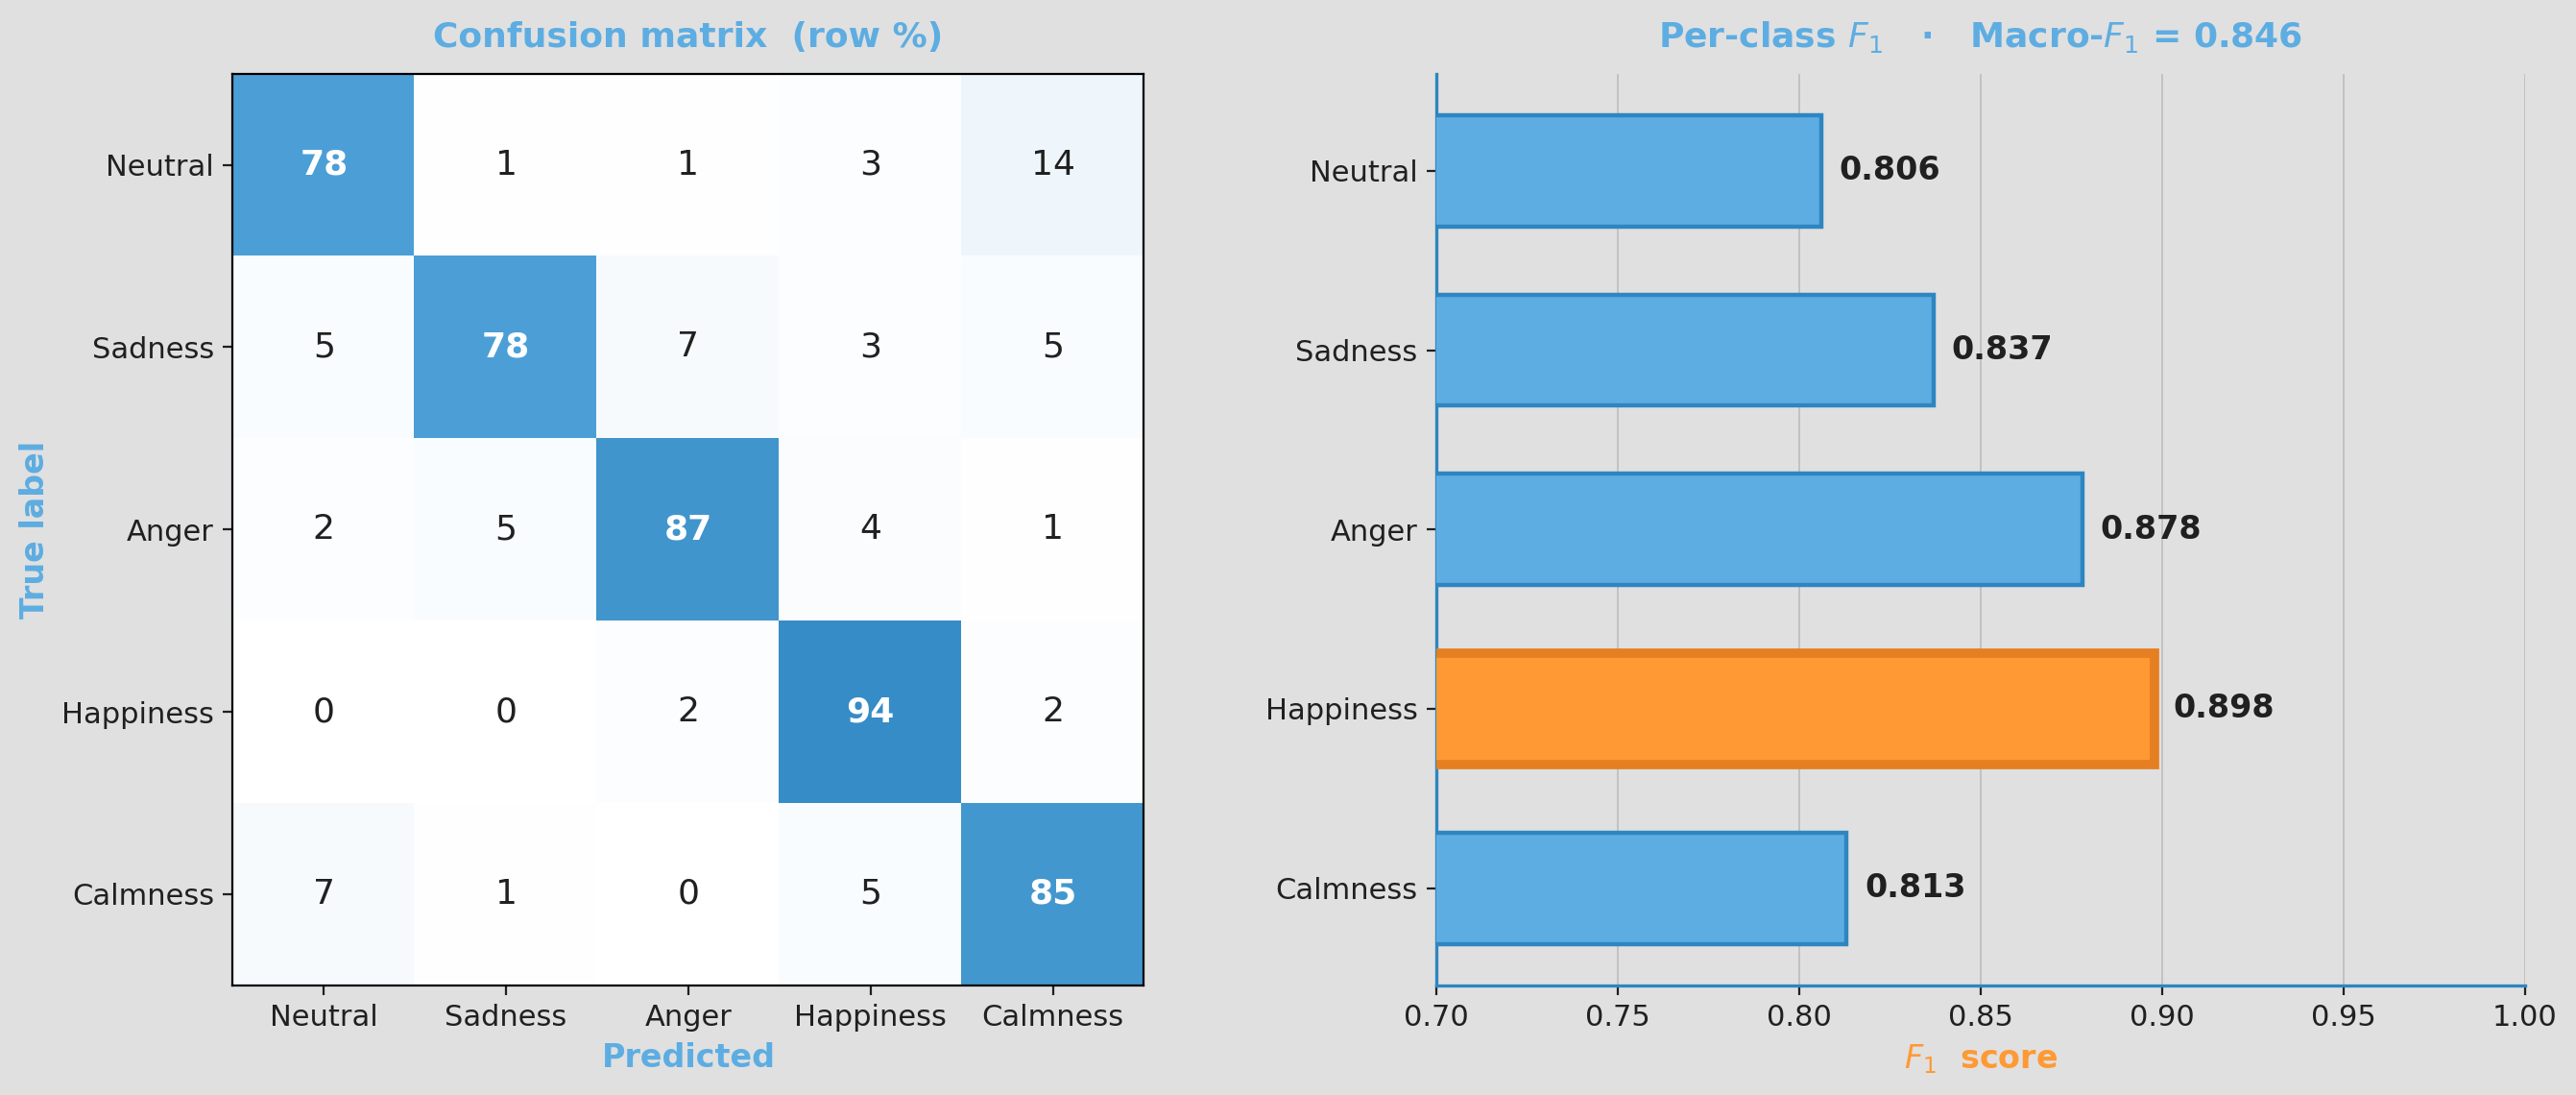
\includegraphics[width=\textwidth]{images/fig_6_4_per_class.png}}{\fbox{\parbox{0.86\textwidth}{\centering Missing image placeholder: \texttt{images/fig\_6\_4\_per\_class.png}.}}}
\caption{Per-class performance of the modality-dropout model on 5{,}040 within-subject test trials, at the Pre-Thesis~II test-selected epoch (absolute values inflated; relative class difficulty only). Left: confusion matrix in row-percent terms. Right: per-class $F_1$.}
\label{fig:per_class_metrics}
\end{figure}

Happiness is the easiest class and Calmness the hardest, with Neutral$\rightarrow$Calmness the largest confusion. The same ordering holds on unseen participants, where the per-class figures are leak-free: Calmness has the lowest recall of the five classes for every method under both normalisations (Table~\ref{tab:cal_perclass}). Calmness is the lowest-arousal positive state in the EAV schema, and it is plausibly hard to separate from Neutral in every modality.

\section{Cross-Modal Coherence}
\label{sec:suppression_matrix}

The Pre-Thesis~II report presented a $5\times5$ suppression matrix at this point and interpreted its dominant cells as population-level patterns of emotion suppression. That analysis, together with the tests showing that its patterns are the error structure of the EEG classifier, is now reported in full in Section~\ref{sec:audit_suppression}.

\section{Comparison with Prior Work on EAV}
\label{sec:eav_prior_comparison}

Only a handful of papers have reported fusion results on EAV \cite{Lee2024EAV} since its 2024 release. Table~\ref{tab:eav_prior_comparison} places the present work beside the three published trimodal fusion methods evaluated on it.

\begin{table}[htbp]
\centering
\caption{Trimodal fusion methods evaluated on EAV. All figures are within-subject. ``n/r'': not reported by the original authors. ``Selection'' records how the reported epoch or checkpoint was chosen, where stated.}
\label{tab:eav_prior_comparison}
\small
\begin{tabular}{p{3.7cm} c c c c c c}
\hline
\textbf{Method} & \textbf{Audio} & \textbf{Vision} & \textbf{EEG} & \textbf{Fusion} & \textbf{Selection} & \textbf{Code} \\
\hline
Lee et al.\ (EAV) \cite{Lee2024EAV}     & 36.7\% & 52.8\% & 36.7\% & ---      & n/r & Yes \\
AMERL \cite{Yin2024AMERL}               & 58.2\% & 67.2\% & 53.5\% & 70.86\%  & n/r & Yes \\
Hyper-MML \cite{Kang2025HyperMML}       & n/r    & n/r    & n/r    & 76.65\%  & n/r & No \\
EEG-MoCE \cite{Anon2026EEGMoCE}         & 60.5\% & 53.8\% & 62.7\% & 75.88\%  & n/r & No \\
\hline
Ours, concat-MLP                        & 57.1\% & 74.6\% & 43.9\% & 79.96\%  & none & Yes \\
Ours, modality dropout                  & 57.1\% & 74.6\% & 43.9\% & 79.80\%  & none & Yes \\
Ours, cross-attention                   & 57.1\% & 74.6\% & 43.9\% & 76.75\%  & none & Yes \\
\hline
\end{tabular}
\end{table}

No state-of-the-art claim is made. The leak-free figures are numerically above the published comparators, but none of the comparators states how its reported epoch or checkpoint was selected, and Section~\ref{sec:audit_selection} shows that on this benchmark that choice alone moves results by 5 to 7.5 points. Chapter~\ref{chap:crosssubject} further shows that within-subject accuracy on EAV is substantially driven by participant identity, which makes within-subject rankings a weak basis for comparing methods. The Pre-Thesis~II claim of a new state of the art (84.7\%) is withdrawn.

Two differences from the comparators remain factual. First, the present work's EEG accuracy (43.9\%) is the lowest among those reported, because vanilla EEGNet \cite{Lawhern2018EEGNet} was retained so that fusion effects are not confounded with a stronger EEG encoder. Second, none of the comparators reports missing-modality robustness, a zero-EEG inference path, a subject-independent evaluation, or a leak-free selection protocol.

\section{Statistical Methodology}
\label{sec:statistical_analysis}

The methods compared in this report produce one accuracy per participant on the same participants, so comparisons are paired. The Wilcoxon signed-rank test \cite{Wilcoxon1945} tests whether the median paired difference is zero without assuming a distributional form; all tests are two-sided. Confidence intervals on means are percentile intervals from 10{,}000 bootstrap resamples of participants \cite{Efron1993Bootstrap}.

Where several tests address one question, the Holm step-down procedure \cite{Holm1979} controls the family-wise error rate within that family, and each table states its family. Holm correction is at least as powerful as Bonferroni correction and makes no assumption about dependence between tests. Families are defined by the question each table answers; where the conclusion depends on the family, as for the within-subject head-versus-naive comparisons, every reasonable family is reported rather than the most favourable one. The naive-late-fusion-versus-vision test of Section~\ref{sec:naive_late_fusion_results} is a single pre-specified test and is not corrected. All tables in Chapters~\ref{chap:within} to~\ref{chap:audit} are produced by \texttt{p3\_stats.py} from the result CSVs.

\section{Discussion}

\textbf{Within-subject, learned fusion adds little over averaging.} Once test-set selection is removed, the best learned heads exceed mean-softmax averaging by about 2.4 points, with a significance that depends on the correction family, and plain attention does not exceed it at all. With 280 training trials per participant, a fusion head has little data from which to learn more than averaging already provides. Chapter~\ref{chap:calibration} identifies the condition under which learned fusion does add value on EAV: an identity-free representation combined with a few dozen labelled clips from the person being recognised.

\textbf{Training discipline matters more than the fusion operator.} The largest reproducible effect among the learned heads is modality dropout ($+3.1$ points for the attention module), not the choice between attention and concatenation, which modality dropout neutralises. The same pattern recurs under subject-independent evaluation.

\textbf{On the EEG performance ceiling.} The 43.9\% mean EEG accuracy reflects EEGNet's performance in EAV's within-subject low-data regime rather than a broken training configuration. With the two training bugs resolved (Chapter~\ref{chap:engineering_challenges}), EEG accuracy exceeds the EAV paper's published 36.7\% baseline. The ceiling is set by the small per-participant training set, the absence of cross-subject EEG pretraining, the non-stationarity of EEG, and how hard it is to separate five emotions in five seconds of 30-channel EEG.

\textbf{On the Listen/Speak asymmetry.} In EAV the EEG segments are taken from the participant's \emph{listening} window and the audio and video from the \emph{speaking} window (Section~\ref{sec:listenspeak_asymmetry}). The three modalities are therefore never simultaneous: a trimodal example pairs the neural response to a cue with the behavioural response to it. This matters little for classification accuracy, but it constrains any trial-level interpretation of agreement between EEG and the audio-visual signals.
